\section{Prise en compte de la mobilité: Blue Banana}
	\label{BlueBanana}
	Il nous a été possible de voir, dans les chapitres précédents, des mécanismes qui permettent de faire évoluer le système en réaction à des événements. En prenant en compte les études des traces des joueurs, Blue Banana a permis de mettre en place un mécanisme d'anticipation des mouvements des avatars pour mieux s'adapter.
	\par Blue Banana présente une solution partielle aux problèmes liés à la mobilité que peut rencontrer une architecture pair à pair dans les MMOGs. La mobilité des avatars implique de nombreux échanges de données à travers le réseau pair à pair, car plus la mobilité est forte plus le nombre de messages de changements de position et de voisin est élevé. Comme les overlays de l'état de l'art n'anticipent pas cette mobilité, les données nécessaires ne seront pas chargées à temps, ce qui conduit à des défaillances transitoires au niveau applicatif. Blue Banana a été réalisé pour résoudre ce problème, il modélise et prédit les mouvements des avatars ce qui permet à l'overlay de s'adapter par anticipation aux besoins du jeux.
	\subsection{Solutions introduites}
	Blue Banana est implémenté au dessus de Solipsis qu'il a été possible d'étudier dans le chapitre~\ref{solipsis}. Il a été possible d'observer plusieurs types de zone (dense ou non, cf.~\ref{trace}) et que les mécanismes d'adaptation sont trop tardifs pour être mis en place dans la réalité (le chargement des données sera trop lent).
	\subsubsection{Les états de l'avatar}
	\label{Automate}
	Une des premières innovations qui a été introduite est la distinction de plusieurs états d'un avatar. Comme il a été possible de voir dans le chapitre sur la collecte de traces, un avatar se comporte différemment en fonction des zones du monde. Trois états ont donc été introduits:
	\begin{itemize}
	\renewcommand{\labelitemi}{$\bullet$}
		\item \textbf{H}(alted): l'avatar est immobile.
		\item \textbf{T}(ravelling): l'avatar se déplace rapidement sur la carte et il a une trajectoire droite.  
		\item \textbf{E}(xploring): l'avatar est en train d'explorer une zone, sa trajectoire est confuse et sa vitesse est lente.
	\end{itemize} 
	Le changement d'état de l'avatar se fait en fonction de la vitesse de celui-ci, si la vitesse devient supérieure à une borne définie et que l'avatar est dans l'état E alors l'avatar passe en état T. Ce modèle pourrait être affiné par la suite en prenant en compte l'accélération ou l'historique des mouvements. Sur la figure~\ref{automateMob}, nous pouvons mieux distinguer les différents changements d'état. Chaque nœud va agir en fonction de cette automate, il sera initialisé à l'état \textbf{H}(alted). \\
	

	\begin{figure}[!h]
        \centering
        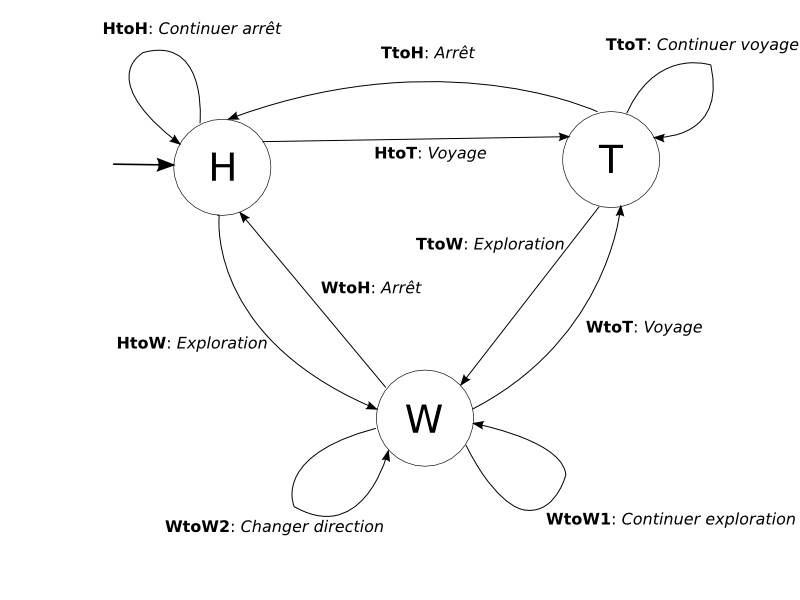
\includegraphics[scale=0.4]{./Ressources/Images/automate.png}
        \caption{\textit{\small Automate décrivant les mouvements d'un avatar. \textbf{En gras}: le nom de la transition, en \textit{italique} sa sémantique}}
        \label{automateMob}
        \end{figure}

\subsection{Le modèle de mobilité}

Un modèle de mobilité a été mis en place dans Blue Banana, nous allons le présenter car il est utilisé pour les différents tests réalisés pour les solutions mises en place. Pour cela, un degré de mobilité à un instant donné, a été introduit. Il s'agit du nombre d'avatars dans l'état \textbf{T}(ravelling) à cet instant sur le nombre total d'avatars. Le modèle de mobilité implémenté dans Blue Banana se base sur l'automate (cf partie~\ref{Automate}). A intervalles réguliers, PeerSim décide si un avatar doit ou non changer d'état. Il réalise ceci grâce aux différentes probabilités présentées dans les fichiers de configurations. A chaque fois qu'un déplacement est décidé, une destination est choisie. L'avatar commence alors son déplacement, chaque mouvement est rectiligne mais non uniforme (car accélération). L'accélération est nulle lorsque la vitesse maximale est atteinte, cette vitesse maximale est choisie en fonction de la zone où se trouve l'avatar.


\par L'automate étant mis à jour toutes les 100ms, même un petit changement dans les probabilités, peut entrainer des gros changements sur la mobilité. La transition WtoT a été choisie, dans Blue Banana, pour faire varier la mobilité. Cette transition permet de déclencher le passage d'un avatar d'un état d'exploration désordonné à un état de déplacement rapide. Sur la figure~\ref{fig:mobility}, nous pouvons voir les différentes valeurs affectées à la transition et les degrés de mobilité correspondants. 

\begin{figure}
  \begin{center}
    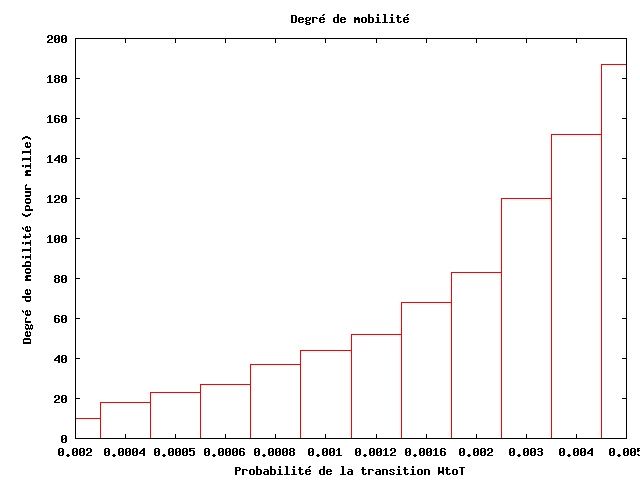
\includegraphics[scale=0.40]{./Ressources/Images/mobility.png} \\
    \caption{\textit{\small Influence du changement de probabilité sur
        la transition WtoT de l'automate sur le degré de mobilité du
        Métavers}}
    \label{fig:mobility}
  \end{center}
\end{figure}






	\subsubsection{Anticipation des mouvements}
	Un autre mécanisme a été mis en place, il s'agit d'anticiper les mouvements d'un avatar, pour cela deux suppositions sont faites: seulement une prédiction courte est cohérente, et plus l'avatar se déplace rapidement, plus il y a de chance qu'il continue dans la même direction~\cite{191}. Comme nous pouvons voir sur la figure~\ref{Propa_Algo}, en fonction du vecteur de mouvement de l'avatar, le nœud B, s'il est dans l'état \textbf{T}, va chercher des nœuds qui se trouvent sur la trajectoire probable de l'avatar, tant que l'ensemble des nœuds préchargés n'est pas plein. Le nœud B va envoyer un message aux voisins qui sont le plus près de lui par rapport au vecteur de mouvement. Un mécanisme pour évaluer si le nœud n'est pas trop près est mis en place. En effet si le temps des communications est supérieur au temps du déplacement de l'avatar, il est inutile de précharger le nœud. Un des risques est de rapatrier des nœuds qui seront inutiles si l'avatar va changer de direction ou d'état. L'amélioration de ce point fait partie des futures pistes pour améliorer l'algorithme d'anticipation des mouvements.\\
	\vspace{5mm}
        \begin{figure}[!h]
        \centering
        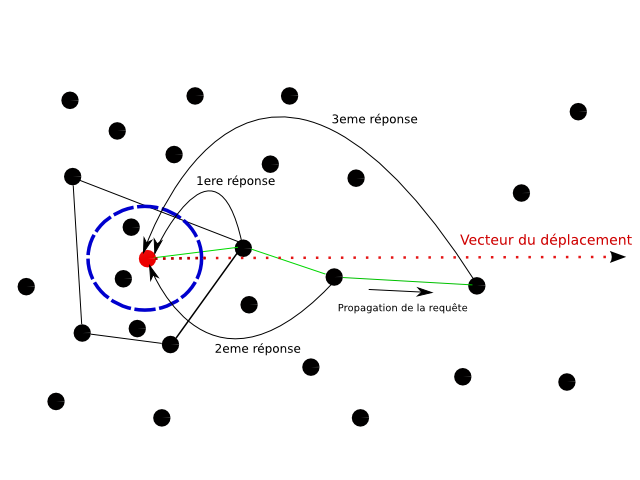
\includegraphics[scale=0.5]{./Ressources/Images/propagation_algo.png}\\
        \caption{Algorithme de propagation}
        \label{Propa_Algo}
        \end{figure}
        \vspace{5mm}
	\subsection{Expérimentations et Résultats}
		Le travail a été testé sur le simulateur à évènements discrets PeerSim ~\cite{peersim}, les expérimentations ont eu pour objectif de comparer Solipsis avec et sans Blue Banana.
		\subsubsection{Le simulateur PeerSim et la description des expérimentations}
		\par PeerSim est un simulateur de réseau pair à pair, qui a deux modes de fonctionnement: par cycles ou par évènements. C'est une API riche et modulaire qui est codée en Java, c'est une composante du projet BISON de l'université de Bologne (Italie). Ce simulateur permet de simuler un large nombre de machines et de tester différentes configurations du réseau. Le simulateur va faire des simplifications sur les couches réseau et les contraintes physiques (latence, pannes, ...). Chaque nœud est considéré comme un module qui va échanger des messages avec les autres nœuds du système. La plupart des plateformes de simulation sont basées sur le modèle à évènements discrets. Il est possible de distinguer deux entités: les nœuds et les messages. Le temps va seulement évoluer à chaque nouvel évènement sur un nœud.
		%\subsubsection{Description des expérimentations}
		\par Au départ de la simulation, une carte initiale des traces est introduite dans le simulateur, la carte provient d'une étude de La et Michiardi~\cite{LM-wosn08} dans Second Life. Ensuite, le simulateur va initialiser l'overlay de Solipsis et vérifier que les deux règles de Solipsis sont bien respectées sur chaque nœud, le reste des traces est ensuite insérer. Il faut aussi régler les différents paramètres du simulateur (nombre d'avatars, taille du monde, densité, accélération des avatars, vitesse de connection, etc). Plusieurs métriques sont mises en place pour évaluer les résultats:
	\begin{itemize}
	\renewcommand{\labelitemi}{$\bullet$}
		\item \textit{Violation des règles fondamentales de  Solipsis}: Regarde si les propriétés de \textit{Global Connectivity} et de \textit{Local Awareness} sont respectées.
		\item \textit{Connaissance des nœuds en avance du mouvement}: Mesure pour les avatars qui se déplacent rapidement, le temps moyen pour qu'il connaisse un nœud qui sera sur sa trajectoire.
		\item \textit{Nombre de messages échangés}: Mesure l'impact de Blue Banana sur le réseau, cela va compter le nombre de messages introduits par Blue Banana et Solipsis.
	\end{itemize}
		\subsubsection{Les résultats}
		Les résultats les plus intéressants montrent que Blue Banana diminue les transitions en échec de 55\% à 20\%, augmentent la connaissance des prochains nœuds de 270\% et cela en créant un overhead de seulement 2\%. Les résultats montrent que le mécanisme d'anticipation introduit par Blue Banana aide l'overlay de Solipsis à s'adapter à temps et à réduire significativement le nombre de violation des règles de Solipsis (de 55\% ou 80\% à 20\%). 
